%%%%%%%%%%%%%%%%%%%%%%%%%%%%%%%%%%%%%%%%%%%%%%
%%%%%%%%%%%%%%%%%%%%%%%%%%%%%%%%%%%%%%%%%%%%%%
%%			     Capitulo 1 			    %%
%%%%%%%%%%%%%%%%%%%%%%%%%%%%%%%%%%%%%%%%%%%%%%
%%%%%%%%%%%%%%%%%%%%%%%%%%%%%%%%%%%%%%%%%%%%%%

\chapter{Introducción} \label{cap1}

Este primer capítulo trata de exponer una breve introducción sobre el problema propuesto, sus antecedentes históricos y los objetivos que se pretenden alcanzar durante el desarrollo de la investigación.

\newpage

%%%%%%%%%%%%%%%%%%%%%%%%%%%%%%%%%%%%%%%%%%%%%%%%%%%%%%%
%		            	Seccion          			  %
%%%%%%%%%%%%%%%%%%%%%%%%%%%%%%%%%%%%%%%%%%%%%%%%%%%%%%%
\section{Propuesta de investigación} \label{s1_1}

Empleados de una oficina, banco o empresa, profesores, alumnos, secretarios, etc. Todos ellos tienen en común que, a diario trabajan con uno o varios ordenadores ya sea para visualizar distintos archivos en cada monitor, realizar diversas tareas agilizando los procesos de cálculo, etc. El proyecto planteado propone un sistema que ofrece la posibilidad de llevar a cabo varias tareas a la vez con diferentes equipos mediante el uso de los mismos dispositivos de control (ratón y teclado) a través de un mecanismo capaz de detectar la orientación del conjunto cabeza-ojos basándose en los movimientos comunes que realiza cualquier persona cuando centra su atención en una u otra pantalla con el propósito de facilitar el trabajo a este tipo de personas, lo cual, incentiva la tarea de investigación. De esta forma, el usuario no trabaja con la incomodidad  de cambiar una y otra vez de teclado y ratón permitiéndole ahorrar espacio en su escritorio debido a que el sistema implementado funciona interpretando estos cambios de posición tan intuitivos. En resumidas cuentas, el usuario dispone de un ratón y teclado convencional con los cuales puede controlar un computador u otro en función del lugar hacia donde dirija su mirada, lo cual, se consigue con un sistema de seguimiento ocular o como se llama comúnmente en inglés, ``eye tracking'' a través del uso de una cámara situada en la pantalla del equipo principal. El sistema se implementa con el objetivo de controlar dos equipos distintos, por tanto, existe una pantalla secundaria que se sitúa a uno de los dos lados. Sin embargo, surgen algunas dudas acerca de este planteamiento como, por ejemplo, si es verdaderamente posible crearlo ya que se desconoce la complejidad de crear un proyecto de tales características. Si se asume la posibilidad de llevarlo a cabo, aparecen otro tipo de cuestiones como qué tipo de hardware es es más ideal para este caso y si existe software libre que ayude a la implementación del código. Como es de esperar, en ingeniería no existen soluciones concretas a determinados problemas sin embargo, la pretensión del proyecto es llevarlo a cabo de la forma mas fiel posible a los objetivos marcados.

%%%%%%%%%%%%%%%%%%%%%%%%%%%%%%%%%%%%%%%%%%%%%%%%%%%%%%%
%		            	Seccion          			  %
%%%%%%%%%%%%%%%%%%%%%%%%%%%%%%%%%%%%%%%%%%%%%%%%%%%%%%%

\section{Antecedentes históricos} \label{s1_2}

Actualmente existe un abanico de soluciones software y hardware para compartir teclado y ratón entre varios ordenadores. En primer lugar, se habla del software KVM (Keyboard Video Mouse) que tiene la finalidad de compartir un teclado y un ratón entre varios equipos sin emplear hardware adicional. Estos proyectos se han llevado a cabo por cuestiones de necesidad y hoy en día, se puede acceder a ellos a través de internet. Algunos de ellos son:

\begin{itemize}
    \item Synergy: Es un software cuyo desarrollador fue Chris Schoeneman. Se trata de una herramienta que permite el uso compartido de un único ratón y teclado para manejar varios ordenadores desde un único escritorio situando el puntero del ratón en el monitor correspondiente. Es open source bajo la licencia de GNU. Dado que no requiere hardware adicional, los equipos se controlan a través del uso de la red de área local. El equipo de Synergy decidió encriptar las conexiones y por tanto, inventaron su propio protocolo sin embargo, no utiliza ningún mecanismo de autentificación ni de cifrado. Además, se trata de un software de pago y es compatible con Windows, Linux y macOS.
    \item Input Director: El autor de este proyecto fue Shane Richards. Este software tiene la misma utilidad que Synergy sin embargo, solo sirve para equipos con el sistema operativo de Windows. El control se realiza de la misma forma que Synergy o incluso con una combinación de teclas que permite cambiar de ordenador. Algunos usuarios prefieren este software frente al anterior debido a que la configuración de este último es más sencilla además de no generar problemas con esclavos que tienen un sistema operativo Windows 7 y ser gratuito.
    \item Multiplicity: Pertenece a la compañía Stardock. La funcionalidad es la misma que los anteriores. Es pago y su tarifa más barata solo permite el control de hasta dos equipos. Ambos ordenadores deben estar conectados en la misma red y únicamente puede instalarse en equipos con Windows 7, 8 y 10.
\end{itemize}

Existe otro tipo de software que ofrece prestaciones similares a los programas descritos, como Across, que utiliza como tecnología de conexión Bluetooth y ShareMouse siendo ambos compatibles con dispositivos Android.

En segundo lugar, existe hardware denominado hardware KVM (KVM switches) que conmuta a un equipo u a otro según una combinación específica de teclas. A estos dispositivos se les conecta los periféricos USB, los conectores VGA, audio y micrófono de los ordenadores que se controlan (entradas del switch) y del monitor principal, altavoces y micrófono, como se muestra en la figura~\ref{fig:switchKVM}.

\begin{figure}[h!]
\centering
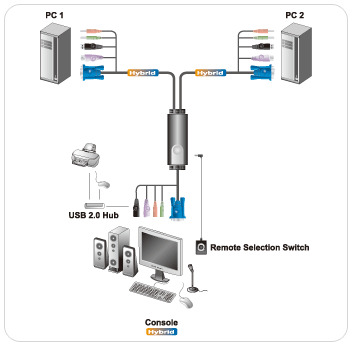
\includegraphics[scale = 0.7]{capitulo_01/figuras_dir/KVM.jpg}
\caption{Control de equipos mediante un switch KVM}
\label{fig:switchKVM}
\end{figure}

En este caso, todos los equipos se controlan a través de una única pantalla. Si se desea usar un monitor por cada equipo independiente, no es necesario que el switch tenga entrada Video. A este hardware se le llama hardware KM.

\begin{figure}
\centering
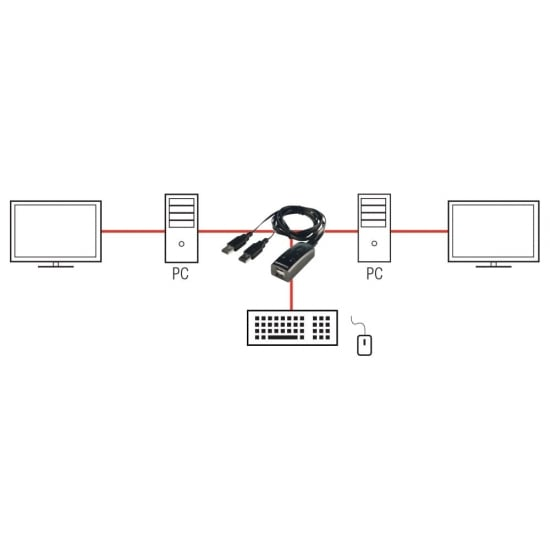
\includegraphics[scale = 0.5]{capitulo_01/figuras_dir/KMSwitch.jpg}
\caption{Switch KM de dos puertos USB. Imagen tomada de Lindy – 2 Port USB KM Switch: https://www.lindy.co.uk/kvm-c6/kvm-switches-c295/2-port-usb-km-switch-p7901}
\label{fig:switchKM}
\end{figure}

Hay varios tipos de hardware KM en función del tipo y del número de conectores y de varias marcas y modelos.

A diferencia de todos los inventos existentes, este proyecto propone un control de equipos mediante el uso de hardware (microcontroladoras) y software (programa desarrolado en C) usando como medio de transimisión la red local vía inalámbrica y el protocolo propio de la red Ethernet (evitando confictos como sucede con Synergy) incorporando un aspecto original como es el control por vista de los equipos mediante periféricos destinados a ese uso. Además, se eliminan problemas de incompatibilidades con el sistema operativo y con los propios dispositivos y la adición de ficheros de código complentario en los distintos equipos para conseguir la correcta comunicación entre el maestro y los esclavos como sucede con algunos de los softwares ya implementados.

%%%%%%%%%%%%%%%%%%%%%%%%%%%%%%%%%%%%%%%%%%%%%%%%%%%%%%%
%		            	Seccion          			  %
%%%%%%%%%%%%%%%%%%%%%%%%%%%%%%%%%%%%%%%%%%%%%%%%%%%%%%%
\section{Definición del problema} \label{s1_3}

Este proyecto engloba tanto hardware como software. En referencia al hardware, se necesita un microcontrolador central que sea capaz de comunicarse con los periféricos. Este dispositivo tiene la función de recoger aquellos datos que envían los dispositivos de control, llamados dispositivos HID o de interfaz humana, para posteriormente enviarlos al correspondiente equipo. A estos datos se les denomina eventos y constituyen tanto pulsaciones de tecla como movimientos del ratón. Este microcontrolador van conectados todos los periféricos, incluidos aquellos que se encargan del seguimiento ocular para obtener los eventos oculares que son usados posteriormente para decidir a qué equipo enviar los eventos HID. Para detectar posición de los ojos (eventos oculares) se necesita una cámara, que en principio, no reúne ninguna característica especial.

Este microcontrolador se comunica con ambos equipos. La comunicación se puede establecer via SPI, I2C, Bluetooth e internet (Wifi o Ethernet), sin embargo, se opta por internet dado que su protocolo es uno de los más conocidos. La forma más sencilla de enviar y recibir datos desde el microcontrolador central es transmitiendo datos a otro microcontrolador que esté conectado a cada uno de los equipos. Dicho lo anterior, el esquema de la figura \ref{fig:esquemahardware} muestra la relación entre los distintos dispositivos involucrados en el proyecto.

\begin{figure}
\centering
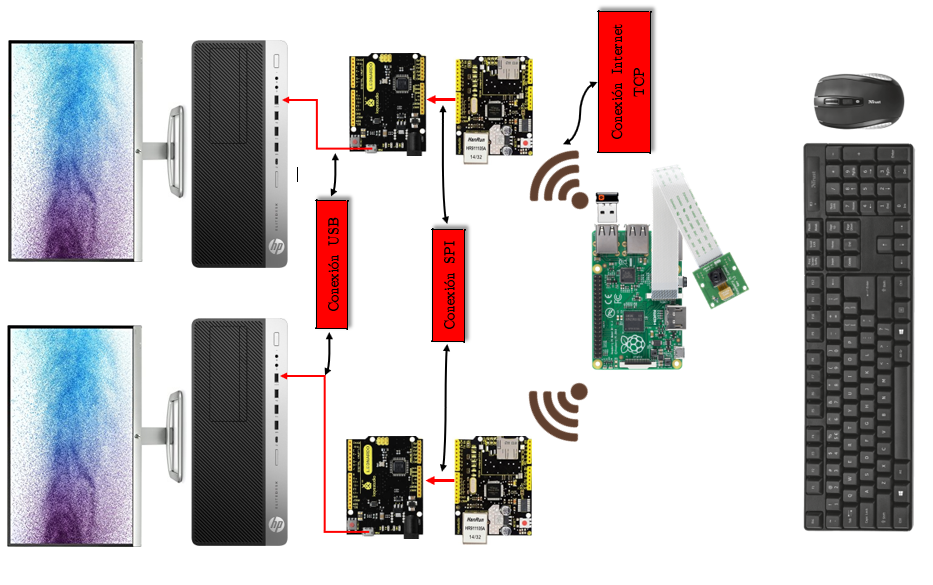
\includegraphics[scale = 0.6, angle=-90]{capitulo_01/figuras_dir/esquemahardware.jpg}
\caption{Esquema del hardware empleado}
\label{fig:esquemahardware}
\end{figure}


Para llevar a cabo lo descrito anteriormente, se necesita implementar la parte software del proyecto. Esta parte engloba un conjunto de programas dedicados a determinadas tareas. En la sección 1.4 a cada una de estas tareas se le asigna un objetivo.

%%%%%%%%%%%%%%%%%%%%% Subsección %%%%%%%%%%%%%%%%%%%%%
\subsection{Estado del arte} \label{s1_3_1}

Existen innumerables combinaciones de dispositivos con los que se podría llegar al objetivo final del proyecto, sin embargo, se puede realizar la selección de dispositivos dando prioridad a ciertos aspectos. La mayoría de los dispositivos que se destacan a continuación son modelos de Arduino o Raspberry Pi debido a que cuentan con una gran comunidad de desarrollo, lo cual facilita enormemente la realización del proyecto.
Se pueden descartar ciertos microcontroladores teniendo en cuenta los tipos de conexión que se pueden establecer entre ellos. Muchos de ellos dificultan el conexionado debido a que no incorporan los conectores correspondientes y por tanto hay que usar módulos adicionales.
Los microcontroladores pueden conectarse entre sí de varias formas permitiendo que uno haga la función de maestro y el resto de esclavos, aunque puede haber excepciones en cuanto al número de maestros. La conexión puede realizarse mediante USB, Bluetooth, SPI, I2C, o mediante red de área local (Ethernet, WiFi).
En la actualidad, ratón y teclado requieren ser conectados mediante USB. Por tanto, el microcontrolador maestro debe disponer de puertos USB. Algunas tarjetas Arduino como “Arduino TRE” y “Arduino Yun” y otras tarjetas Raspberry Pi como el modelo antiguo “Raspberry Pi 1 A” traen incorporado un solo conector USB. Esta característica podría ser válida en el caso de disponer de un teclado y un ratón inalábricos con un único módulo USB. Si se dispone de los periféricos por separado, esta solución no es la más recomendable debido a que se necesita una tarjeta complemetaria o shield como por ejemplo “Arduino USB Host Shield” o similar para aumentar el número de conectores USB. Hay que tener en cuenta también que el microcontrolador maestro debe conectarse de alguna forma a los microcontroladores esclavo. La conexión entre ambos puede llevarse a cabo mediante bluetooth. Existen algunas placas Arduino que incorporan esta funcionalidad como son “Arduino 101”, “Arduino BT” y “Arduino Primo” o de Raspberry como el modelo “3 B” y también, para todas aquellas que no tengan este tipo de conexión, existe un módulo bluetooth como “HC-05”. Sin embargo, estas placas Arduino no disponen de puertos USB, luego quedan descartables. Otra opción consiste en usar la conexión SPI. Es una conexión disponible en la mayoría de los microcontroladores que permite la transmisión serie de los datos y es más rápida que la I2C. El dispositivo maestro debe contar con tantas líneas “Slave Select” como ordenadores estén conectados en el sistema (o número de esclavos) por tanto, este hecho supone una limitación en cuanto al número de dispositivos conectados en el sistema. Los esclavos pueden tener una sola entrada “SS” por tanto, en este aspecto podría ser últil una placa “Teensy” o casi cualquier placa Arduino. No sucede lo mismo si la se conectan mediante I2C ya que todos los dispositivos están conectados a dos líneas de comunicación únicamente sin necesitar un puerto a parte para controlar el envío de datos a cada esclavo. Casi cualquier placa soporta este tipo de conexión, no obstante, los datos se transmiten por una sola línea que permite que el esclavo y el maestro se comuniquen, es decir, es un protocolo half-duplex. Esto significa que ocurren conflictos cuando uno envía un 1 lógico y el otro, un 0 lógico al mismo tiempo. Existen soluciones a esto, como conectar a ambas líneas resistencias pull-up pero con la finalidad de simplificar el problema, se puede acudir a la conexión por red descartando por completo la conexión UART ya que es asíncrona, la velocidad de transferencia está limitada y es una conexión punto a punto y por tanto solo puede haber dos dispositivos conectados a una misma línea. En caso de emplear la conexión por red, se consigue una serie de ventajas frente al resto de protocolos de comunicación como la mayor velocidad de transferencia, el número ilimitado de esclavos que se pueden comunicar con el maestro y la no intervención de elementos de conexión físicos. Algunos microcontroladores como “Teensy” o “Nano” de Arduino no incluyen la posibilidad de conectarse a la red. Sin embargo, existe un modelo de Raspberry Pi que tiene la opción de comunicarse con otros dispositivos por vía wifi llamado “Raspberry Pi Zero W”.
En resumen, la mejor opción vista hasta ahora como dispositivo maestro es la “Raspberry Pi 3 Model B” ya que dispone de cuatro puertos USB para conectar los periféricos y conexión Wifi y Ethernet para comunicarse con el dispositivo esclavo. A su vez, es una buena idea que este último sea un Arduino Leonardo (ya que su microcontrolador permite simular eventos HID) con un módulo ethernet o wifi que le permite conectarte mediante Wifi o ethernet al maestro y mediante USB, al ordenador correspondiente además de ser ambos microcontroladores que cuentan con una amplia comunidad de desarrollo y se puede trabajar con código abierto, es decir, código distribuido libremente de fácil acceso y con la posibilidad de modificarlo sin restricciones.


%%%%%%%%%%%%%%%%%%%%%%%%%%%%%%%%%%%%%%%%%%%%%%%%%%%%%%%
%			Seccion				                      %
%%%%%%%%%%%%%%%%%%%%%%%%%%%%%%%%%%%%%%%%%%%%%%%%%%%%%%%
\section{Objetivos del proyecto y resultados esperados} \label{s1_4}

El objetivo principal del proyecto consiste en realizar el prototipo del sistema basado en el hardware descrito en la sección 1.3 y el software implementado a lo largo de la investigación que permita conseguir el control de dos equipos distintos con los mismos dispositivos de interfaz humana mediante un mecanismo de seguimiento ocular tal y como se menciona en la sección 1.1. 

El objetivo principal puede conseguirse siempre y cuando se logre implementar los programas correspondientes a cada una de estas etapas que compone la tarea de investigación que constituyen los objetivos secundarios del proyecto:
\begin{itemize}
    \item Obtención y demultiplexado de los eventos del teclado y del ratón.
    \item Corrección de la distorsión radial de la cámara.
    \item Obtención de los eventos oculares.
    \item Envío de los eventos de dispositivos HID a los microcontroladores secundarios (microcontroladores Arduino Leonardo).
    \item Configuración de Raspberry Pi Zero como cliente de la comunicación vía internet.
    \item Simulación de los eventos recibidos como pulsaciones de teclas y movimientos del ratón.

\end{itemize}

%%%%%%%%%%%%%%%%%%%%%%%%%%%%%%%%%%%%%%%%%%%%%%%%%%%%%%%
%			Seccion				                      %
%%%%%%%%%%%%%%%%%%%%%%%%%%%%%%%%%%%%%%%%%%%%%%%%%%%%%%%
\section{Metodología de la investigación y organización de la memoria} \label{s1_5}

La consecución de los objetivos fijados es posible bajo la dirección de Francisco Moya Fernández, quien ha facilitado documentación de ayuda mediante su libro ``Taller de Raspberry Pi''. Con él, pretende familiarizar a los alumnos con todo aquello relacionado con el entorno de Linux. El libro consta de varias secciones que tratan diversos temas de interés. Una de las secciones más relevantes en el proyecto trata sobre la biblioteca ``Reactor'' que ha sido fundamental en el desarrollo del programa de lectura y demultiplexado de eventos de dispositivos HID haciendo uso de manejadores de tipo ``event handler'' como se describe en secciones posteriores del documento. El programa del taller de Raspberry Pi no sólo incluye el libro anterior sino que presta un microcontrolador Raspberry Pi para el desarrollo de software en el entorno de Raspbian, un sistema operativo basado en Debian. El libro del taller recomienda además el uso de un sistema de control de versiones o GIT, que mantiene un registro de todas las modificaciones que se realizan sobre un programa tras el ``comiteado'' del archivo\footnote{Para más información, véase el libro Git Pro \citep{GIT}}. De esta forma, se evitan problemas por pérdida de información debida a defectos en sectores del disco duro o incluso la rotura total del mismo ya que todas las versiones se almacenan en la nube.

Junto a las explicaciones y bibliografía aportadas por el director del proyecto, la comunidad de desarrollo de software libre ayuda enormemente la tarea de investigación. Además, se ha establecido como metodología de planificación la llamada ``planificación ágil''. Consiste en conocer los requisitos del cliente y en base a ello, crear las llamadas ``historias de usuario'' que constituyen las tareas a realizar para satisfacer los requisitos que el cliente impone sobre el producto. El director del proyecto actúa como cliente, decidiendo qué requisitos son los más importantes y entre ambos, se realiza una estimación del tiempo a invertir en cada historia. Posteriormente, en función de la prioridad que otorgue el director a las historias de usuario, se agrupan formando iteraciones de duración total entre una y dos semanas. El resultado de esas iteraciones debe ser algo claramente apreciable por el cliente.

Respecto a la memoria, se divide principalmente en cuatro bloques: conceptos teóricos, procedimientos, resultados y conclusiones. A su vez, los tres primeros están formados por las secciones relativas a los objetivos secundarios, ya que la realización de todos ellos supone la finalización del proyecto.

